\documentclass[10pt, oneside, reqno]{amsbook}
\usepackage{amsthm, amsmath, amssymb}
\usepackage{setspace, graphicx, enumerate}
\onehalfspacing    
\usepackage{fontspec,xltxtra,xunicode}
\defaultfontfeatures{Mapping=tex-text}



% AMS Theorems
\theoremstyle{plain}% default 
\newtheorem{thm}{Theorem}[chapter] 
\newtheorem{lem}[thm]{Lemma} 
\newtheorem{prop}[thm]{Proposition} 
\newtheorem{exer}[thm]{Exercise} 
\newtheorem*{cor}{Corollary} 


\newcommand{\res}[2]{\text{Res}(#1,#2)}
\theoremstyle{definition} 
\newtheorem{defn}[thm]{Definition}
\newtheorem{conj}[thm]{Conjecture}
\newtheorem{exmp}[thm]{Example}

\theoremstyle{rem} 
\newtheorem*{rem}{Remark} 
\newtheorem*{note}{Note} 
\newtheorem{case}{Case} 
\theoremstyle{definition}
\newtheorem{dfn}[thm]{Definition}

%\newtheorem*{remu}{Remark}
\newtheorem{ex}[thm]{Example}
\newtheorem{exs}[thm]{Examples}

\newtheorem{metaphor}{Metaphor}
\newtheorem{idea}{Idea}
\newtheorem{convention}{Convention}
\newtheorem{recall}{Recall}
\def \grad {\overrightarrow{\nabla}}
\def \curl {\overrightarrow{\nabla} \wedge \cdot}
\def \div {\overrightarrow{\nabla} \cdot}
\def \nab {\ensuremath{\nabla}}
\def \im {\text{im }}
\def \ker {\text{ker }}
\def \scal {\text{<\textperiodcentered,\textperiodcentered>}}
\newcommand{\scalprod}[2]{\langle #1,#2 \rangle}


\def \Ccal {\ensuremath{\mathcal{C}}} % for categories
\def \D {\ensuremath{\mathcal{D}}}
\def \S {\ensuremath{\mathcal{S}}}
\def \P {\ensuremath{\mathcal{P}}}
\def \U {\ensuremath{\mathcal{U}}}
\def \H {\ensuremath{\mathcal{H}}}
\def \psiket {\ensuremath{|\psi \rangle}}
\def \phiket {\ensuremath{|\phi \rangle}}
\def \psibra {\ensuremath{\langle \psi |}}
\def \phibra {\ensuremath{\langle \phi |}}

\usepackage{textcomp}
\def\Cbb{\ensuremath{\mathbb{C}}}
\def\Kbb{\ensuremath{\mathbb{K}}}
\def\Nbb{\mathbb{N}}
\def\Pbb{\ensuremath{\mathbb{P}}}
\def\Qbb{\ensuremath{\mathbb{Q}}}
\def\Rbb{\ensuremath{\mathbb{R}}}

\def \eps {\varepsilon}
\def \AA{\ensuremath{\mathcal{A}^{1}}}
\def  \AAA{\ensuremath{\mathcal{A}}}
\def \Fff{\mathfrak{F}}
%\def \commutes {\ar@{}[rd]|{\circlearrowleft}}
\def \commutes {\ar@{}[rd]|{\mbox{ \Large{$\circlearrowleft$} }}}
\def\dx{\,\mathrm dx}
\newcommand{\tensor}{\otimes}
\newcommand{\gt}{>}
\newcommand{\lt}{<}
\newcommand{\itexarray}[1]{\begin{matrix}#1\end{matrix}} %To draw commutative Diagrams
\newcommand{\Ob}{{\rm Ob}}
     \newcommand{\Cob}{{\rm Cob}}   
	\newcommand{\Vect}{{\mathrm{Vect}}}   
	\newcommand{\Hilb}{{\mathrm{Hilb}}}    
	\newcommand{\tr}{{\rm tr}}   
      \newcommand{\Hom}{{\rm hom}}
\newcommand{\cChVect}{\mathrm {cCh(Vect)}}
\newcommand{\gVect}{\mathrm {gVect}} 
\newcommand{\To}{\ensuremath{\rightarrow \;}}  
\newcommand{\newword}[1]{\textbf{\emph{#1}}}
\newcommand{\eee}{\ensuremath{e_{i_1}\wedge \cdots \wedge e_{i_p}}}
\def \hodge{*}
\def \iso {\cong}
\newcommand{\expc}[1]{\mathbb{E}\left[#1\right]}
\newcommand{\var}{\text{Var}}
\newcommand{\cov}[1]{\text{Cov}\left(#1\right)}
\newcommand{\prob}[1]{\mathbb{P}(#1)}
\newcommand{\given}{ \, | \,}
\newcommand{\us}{0 \leq u \leq s}
\newcommand{\ts}[1]{\{ #1 \}}

\renewcommand{\phi}{\varphi}
\newcommand{\sigf}{\mathcal{F}}

\newcommand{\dzz}{\, dz}
\newcommand{\bigo}[1]{\mathcal{O}(#1)}

\newcommand{\al}{\alpha}
\newcommand{\Q}{\mathbb{Q}}
\newcommand{\R}{\mathbb{R}}
\newcommand{\C}{\mathbb{C}}
\newcommand{\Z}{\mathbb{Z}}
\newcommand{\E}{\mathbb{E}}
\newcommand{\N}{\mathbb{N}}

\newcommand{\I}{\mathbb{I}}

\renewcommand{\P}{\mathbb{P}}

\newcommand{\F}{\mathbb{F}}
\newcommand{\Ga}{\mathbb{G}}

\newcommand{\aut}[1]{\text{Aut}{(#1)}}

\newcommand{\gener}[1]{\langle #1 \rangle}
\newcommand{\charr}[1]{\text{char}(#1)}
\newcommand{\nth}{n\textsuperscript{th}}

% \newcommand{\limsup}{\text{limsup}}

\newcommand{\tworow}[2]{\genfrac{}{}{0pt}{}{#1}{#2}}
\newcommand{\xdeg}[2]{[#1 : #2]}
\newcommand{\gal}[2]{\text{Gal}(#1/#2)}
\newcommand{\minpoly}[2]{m_{#1, #2}(x)}

\newcommand{\mapping}[5]{\begin{align*}
    #1 : \quad     #2 &\rightarrow #3 \\
            #4  &\mapsto #5
\end{align*}    
}


\def\cip{\,{\buildrel p \over \rightarrow}\,} 
\def\cid{\,{\buildrel d \over \rightarrow}\,} 
\def\cas{\,{\buildrel a.s. \over \rightarrow}\,} 

\def\clp{\,{\buildrel L^p \over \rightarrow}\,} 

\def\eqd{\,{\buildrel d \over =}\,} 
\def\eqas{\,{\buildrel a.s. \over =}\,}
\newcommand{\sigg}{\mathcal{G}}     
\newcommand{\indic}[1]{\mathbf{1}_{\{ #1 \}} }
\newcommand{\ito}{It\^o\ }      
\newcommand{\itos}{It\^o's\ }       

\newcommand{\doleans}[1]{\mathcal E_t \left(\int_0^\cdot #1 \right)}

\numberwithin{equation}{chapter}

\usepackage{hyperref}
        
\title{Interest Rate Modelling}                              % Document Title
\author{Peadar Coyle}
%\date{}                                           % Activate to display a given date or no date


\begin{document}

\maketitle \tableofcontents \clearpage


\tableofcontents

\chapter{Preliminaries} % (fold)
\label{cha:preliminaries}

% chapter preliminaries (end)
\section{Introduction to Interest Rate Modelling} % (fold)
\label{sec:introduction_to_interest_rate_modelling}

% section introduction_to_interest_rate_modelling (end)
There is a one-to-one correspondence between the class $Q$ of all probability measures equivalent to $\P$ and the class $\Lambda$ of all $\F$-adapted (or $\F$-predictable) process $\lambda_t$ satisfying \[
    \P\left(\int_0^{T^\star} |\lambda_u|^2 \, du < \infty \right) = 1
\]
and \[
    \E_\P\left( \mathcal{E}_{T^\star} \left(\int_0^\cdot \lambda_u \, dW_u\right) \right) = 1
\] 
Thus our correspondence is \[Q \ni \P^\lambda \iff \lambda \in \Lambda.\]
Consequently, \begin{enumerate}[(i)]
    \item $\frac{d\Q}{d\P} = \eta_{T^\star}$
    \item \begin{align*}
        \frac{d\Q}{d\P} \given \sigf_t  &= \eta^\Q_t \\
                                        &= \E_\P\left(\eta_{T^\star} \given \sigf_t \right) \\
                                        &= \doleans{\lambda_u \, dW_u}
    \end{align*}
\end{enumerate}

\begin{thm}[Abstract Bayes formula]
    Let $\Q \sim \P$ with $\frac{d \Q}{d \P} = \eta$.  Suppose that $\sigg \subset \sigf$.  We then have \[
        \E_\Q(X \given \sigg) = \frac{\E_\P(\eta X \given \sigg)}{\E_\P(\eta \given \sigg)}.
    \]  Note that is $\sigg = \{ \emptyset, \Omega \}$ then the formula reduces to \[
        \E_\Q(X) = \E_\P(\eta X).
    \]

    If $Q \sim \P$ with $\frac{d\Q}{d\P} |_{\sigf_t} = \eta_t$, for all $t \in [0, T^\star]$, then \[
        \E_\Q(X \given \sigf_t) = \frac{\E_\P(\eta_{T^\star} X \given \sigf_t)}{\E_\P(\eta_{T^\star} \given \sigf_t)}.
    \]
    
    Hence if $X$ is $\sigf_t$ measurable for some $T \in [0, T^\star]$ then \[
        \E_\Q(X \given \sigf_t) = \frac{\E_\P(\eta_T X \given \sigf_t)}{\eta_t} = \E_\P(\eta_t^{-1} \eta_T X \given \sigf_t)
    \]
\end{thm}

\begin{exmp}
    If $\eta_t = \doleans{\lambda_u \, dW_u}$, then \[
        \E_\Q(X \given \sigf_t) = \E_\P(e^{\int_t^T \lambda_u \, dW_u - \frac{1}{2} \int_0^t |\lambda_u|^2 \, du} X \given \sigf_t)
    \] 
\end{exmp}


\begin{lem}
    \label{lem:martingale_equivalence_measures}
    A $\F$-adapted and $\Q$-integrable process $M$ is a $(\Q, \F)$-martingale if and only if the product $M \eta$ is a $(\P, \F)$-martingale.
\end{lem}

\begin{proof}
    $\E_\Q(M_t \given \sigf_s) = M_s$, $s \leq t$, so \[
        M_s = \E_\Q(M_t \given \sigf_s) = \frac{\E_\P(\eta_t M_t \given \sigf_s)}{\eta_s}
    \]
\end{proof}

\begin{lem}
    If $X$ and $Y$ are two processes of the form \begin{align*}
        dX_t &= \alpha_t \, dt + \beta_t \, dW_t \\
        dY_t &= \tilde \alpha_t \, dt + \tilde \beta_t \, dW_t
    \end{align*} then the product satisfies the \ito product formula \begin{align*}
        d(X_t Y_t) = X_t \, dY_t + Y_t \, dX_t + d \langle X, Y \rangle_t
    \end{align*}    
\end{lem}

If $X$ is of the form $dX_t = \alpha_t \, dt + \beta_t \, dW_t$ and $f$ is of class $C^2(\R)$, then the continuos martingale part of $Y_t = f(X_t)$ is given as \[
    \int_0^t f'(X_u) \beta_u \, dW_u
\]

\begin{prop}
    \label{prop:proposition_1.1}
    % TODO MUST COMPLETE - PROPOSITION 1.1 in course notes.
\end{prop}

\begin{proof}[Proof of Proposition 1.1]
    Let $\P^\lambda$ be equivalent to $\P$, so that \[
        d\eta_t = \eta_t \lambda_t \, dW_t
    \]  and \[
        \frac{d\P^\lambda}{d \P} = \eta_t
    \] on $(\Omega, \sigf_t)$, $t \in [0, T^\star]$.

    Define $B(t, T)$ as follows, for all $t \in [0, T]$, \begin{align*}
        B(t, T) &= B_t \E_{\P^\lambda} \left( \frac{1}{B_T} \given \sigf_t \right) \\
        &= \E_{\P^\lambda} \left(e^{-\int_t^T r_u \, du} \given \sigf_t \right)
    \end{align*}
    
    For i), we simply apply Girsanov's theorem, replacing $dW_t$ by $dW_t = dW^\lambda_t - \lambda_t \, dt$ in the dynamics of $r$ under $\P$.  
    
    For ii), we first recall that $Z(t, T) = \frac{B(t, T)}{B_t}$ is given by \[
        Z(t, T) = \E_{\P^\lambda} \left( \frac{1}{B_T} \given \sigf_t \right)
    \] is a $(\P^\lambda, \F)$-martingale.
    
    Note that $\F^{\lambda} \neq \F$ in general.  From Lemma \ref{lem:martingale_equivalence_measures}, we know that $\eta_t Z(t, T)$ is a $(\P, \F)$-martingale.  Thus applying the predictable representation property, there exists an $\F$-adapted process $\gamma_t$ such that \[
        M_t \equiv \eta_t Z(t, T) = Z(0, T) + \int_0^t \gamma_u \, dW_u
    \] for all $t \in [0, T]$.  Consequently, $dM_t = \gamma_t \, dW_t$ and hence \[
        dZ(t, T) = d(\eta^{-1}_t M_t) = M_t \, d\eta_t^{-1} + \eta_t^{-1}\, dM_t + d \langle \eta^{-1}, M \rangle_t
    \]  where \begin{align*}
        d \eta_t^{-1} = - \eta_t^{-1} \lambda_t \, dW_t^\lambda.
    \end{align*}  We obtain \begin{align*}
        dZ(t, T) &= \eta_t Z(t, T) \left( - \eta_t^{-1} \lambda_t \, dW_t^\lambda \right) + \eta_t^{-1} \gamma_t \left(dW_t^\lambda + \lambda_t \, dt \right) + \left(- \eta_t^{-1} \lambda_t \gamma_t \right) \, dt \\
        &= \eta_t^{-1} \left(\gamma_t - M_t \lambda_t \right) \, dW_t^\lambda
    \end{align*} so that \[
        dZ(t, T) = \tilde b^\lambda(t, T) \, dW_t^\lambda
    \]  Since $B(t, T) = B_t Z(t, T)$, using again the \ito formula we have \begin{align*}
        dB(t, T)    &= B_t \, dZ(t, T) + Z(t, T) \, dB_t  \\
                    &= \frac{B(t, T)}{B_t} r_t B_t \, dt + B_t \tilde b^\lambda(t, T) \, dW_t^\lambda \\
                    &= r_t B(t, T) \, dt + B(t, T) \underbrace{\frac{B_t \tilde b^\lambda(t, T)}{B(t, T)}}_{b^\lambda(t, T)} \, dW^\lambda_t.
    \end{align*}   We conclude that for all $T \in [0, T^\star]$, there exists an $\F$-adapted process $b^\lambda(t, T)$, $t \in [0, T]$ called the volatility of the bond
, such that \[
    dB(t, T) = B(t, T)(r_t \, dt + b^\lambda(t, T) \, dW^\lambda_t).  
\]    In fact, it does not depend on the choice of $\lambda$.  For simplicity, we can write $b(t, T) \equiv b^\lambda(t, T)$.  

The final formula is a special case of the well known result:
\begin{align*}
    dX_t    &= X_t (\alpha_t \, dt + \beta_t \, dW_t) \\
                \Updownarrow  \\
        X_t &= X_0 e^{\int_0^t \alpha_u \, du} \doleans {\beta_u \, dW_u }  \\
            &= X_0 e^{\int_0^t \alpha_u \, du} e^{\int_0^t \beta_u \, dW_u - \frac{1}{2} \int_0^t |\beta_u|^2 \, du}
        \end{align*}
        
    This completes our proof of Proposition 1.1, under the assumption that $\frac{1}{B_T}$ is $\P^\lambda$-integrable.
    % We have \[
    %   dM_t = \eta_t \lambda_t dW_t
    % \] and \[
    %   dM_t^{-1} = - \eta_t^{-1} \lambda_t dW^\lambda_t.
    % \]  This is true as \[
    %   \frac{d\P}{d\Q}
    % \]
\end{proof}

There are still several issues given this pricing formula. 
\begin{enumerate}[(i)]
    \item How to compute $b(t, T)$ explicitly in terms of $\mu$ and $\sigma$ under the assumptions that \[
        dr_t = \mu(r_t, t) \, dt + \sigma(r_t, t) \, dW_t
    \] and $\lambda_t = \lambda(r_t, t)$ is the risk premium.  
    \item How can we calibrate our short-term rate model, meaning that \[
        \E_{\P^\lambda}\left( \frac{1}{B_T} \right) = B(0, T) = P(0, T).
    \]
\end{enumerate}  

The issue of pricing bonds is related to solving a backward stochastic differential equation (BSDE).  The general form is \[
    X_t = X_0 + \int_0^t \mu (X_u, u) \, du + \int_0^t \xi_u \, dW_u \tag{$\star$}
\]   where $\mu : \R \times \R^+ \rightarrow \R$ is some function and $\xi$ is some $\F$-adapted process.  We also fix $T > 0$ and postulate that $X_T$ is a \textbf{known } $\sigf_T$-measurable random variable. 

\begin{defn}
    We say that $(X, \xi)$ solves the BSDE with terminal condition with terminal condition $Y$ ($\sigf_T$-measurable) if: 
    \begin{enumerate}[(i)]
        \item $(X, \xi)$ satisfies ($\star$), 
        \item $X_T = Y$.  
    \end{enumerate}
    
    This can be extended to cases where $\mu : \R \times \R^+ \times \Omega \rightarrow \R$ is $\F$-adapted.
\end{defn}


\chapter{Markovian Models of the Short Rate} % (fold)
\label{cha:markovian_models_of_the_short_rate}

    Let $\P^\star$ be a martingale measure in the sense that \[
        B(t, T) = \E_{\P^\star} \left( e^{-\int_t^T r_u \, du} \given \sigf_t \right).
    \]  In particular, \[
        B(0, T) = \E_{\P^\star} \left( e^{-\int_0^T r_u \, du}  \right).  
    \]  We postulate that \begin{equation}
        dr_t = \mu(r_t, t) \, dt + \sigma(r_t, t) \, dW^\star_t,
        \label{eq:generic_short_rate}
    \end{equation} where $W^\star$ is a Brownian motion under $\P^\star$. The filtration $\F$ is any filtration such that $W^\star$ is a BM with respect to $\F$ .  We assume that \eqref{eq:generic_short_rate} has a unique (strong) solution. 
    
    Then it known that $r_t$ has the Markov property with respect to $\F$, meaning that for any bounded continuous function $h : \R \rightarrow \R$, \[
    \E_{\P^\star} \left(h(r_t) \given \sigf_s \right) = \E_{\P^\star}\left(h(r_t) \given r_s \right)
 \] for all $s \leq t$.   

Hence \[
    \E_{\P^\star} \left(e^{-\int_t^T r_u \, du} \given \sigf_t \right) = v(r_t, t, T) = \tilde v(r_t, t) 
\] suppressing the dependence on $T$.

Goals:
\begin{enumerate}[(i)]
    \item Compute explicitly $v(r_t, t, T)$ for some classical models \begin{enumerate}[(a)]
        \item Merton's model 
        \item Vasicek's model
        \item CIR model (Bessel process)
    \end{enumerate}
    using either the probabilistic approach (martingale measure) or the  analytic approach (PDEs).
    \item Represent the price of the bond as follows \[
        B(t, T) = \exp \left( m(t, T) - n(t, T) r_t \right)
    \]
    
    For a fixed maturity $T$, \[
        m(\cdot, T), n(\cdot, T) : [0, T] \rightarrow \R
    \] can also be computed using the second method by separating variables in the PDE.  Note that $m(T, T), n(T, T) = 0$.
    \item Compute explicitly the volatility $b(t, T)$ of the bond by applying the \ito formula to the function $v(r_t, t, T)$.
    \item Extend the model to the time-inhomogenous case in order to ensure that $B(0, T) = P(0, T)$ for all $T \in [0, T^\star]$.
\end{enumerate}

\section{Merton's model} % (fold)
\label{sub:merton_s_model}
    Assure \[
        r_t = r_0 + at + \sigma W_t^\star 
    \] where $W^\star = W^\lambda$ for some $\lambda$.  Hence
    \begin{equation}
        dr_t = a \, dt + \sigma \, dW^\star_t, \quad r_0 > 0.
    \end{equation} 
    \begin{note}
        The generator of the time homogenous Markov diffusion can be represented as \[
            A_r = a \frac{\partial }{\partial r} + \frac{1}{2} r^2 \frac{\partial^2}{\partial r^2}.  
        \]
    \end{note}

    \begin{prop}
        The price $B(t, T)$ is given by \begin{equation}
            \label{eq:merton_short_rate_price}
            B(t, T) = e^{-r_t(T-t) - \frac{1}{2}a(T-t)^2 + \frac{1}{6} \sigma^2(T-t)^3}.  
        \end{equation}  Hence \[
            dB(t, T) = B(t, T)\left(r_t \, dt - \sigma(T-t) dW^\star_t \right).
        \]  Thus we have the volatility of the bond $b(t, T) = -\sigma(T-t)$.
    \end{prop}
    
    \begin{proof}
        It is enough to calculate $B(0, T)$ and then establish the general formula for $B(t, T)$ using the property that $r_t$ is a time-homogenous Markov process, thus \[
            B(0, T) = v(r_0, T) \Rightarrow B(t, T) =v(r_t, T-t)
        \]
        Computation of $B(0, T)$ is done as follows:\[
            B(0, T) = \E_{\P^\star} \left(e^{-\int_0^T r_u \, du} \right) = \E_{\P^\star} \left( e^{-\xi_T} \right)
        \] where the distribution of $\xi_T$ can be found explicitly.  We argue that \[
            \xi_T \sim N\left(r_0 T + \frac{1}{2} a T^2, \frac{1}{3} \sigma^2 T^3 \right)
        \]  We have \begin{align*}
            \xi_T   &= \int_0^T r_u \, du \\
                    &= \int_0^T \left( r_0 + au + \sigma W^\star_u \right) \, du \\
                    &= \int_0^T (r_u + au)  \, du + \sigma \int_0^T W^\star_u \, du
        \end{align*}
        Th rest proceeds quite simply.
        
        We then derive the dynamics of $B(t, T)$.  By the \ito formula, we have that since $B(t, T) = v(r_t, t, T)$, we must have \[
            dB(t, T) = r_t B(t, T) \, dt + b(t, T) B(t, T) \, dW^\star_t.  
        \] Note that the martingale component comes from \[
            \frac{\partial v}{\partial r} dr_t 
        \] and \[
            \frac{\partial}{\partial r}v(r_t, t, T) = -(T- t) v(r_t, t, T)
        \] so that \begin{align*}
            \frac{\partial}{\partial r}v(r_t, t, T) \, dr_t &= -(T-t) v(r_t t, T) (a \, dt + \sigma \, dW^\star_t) \\
            &\sim - \sigma(T- t)B(t, T) \, dW^\star_t
        \end{align*}  We then obtain the equality $B(t, T) = -\sigma(T-t)$.  In particular, $B(t, T) = 0$.  
    \end{proof}
    
    \begin{exer}
        Apply the PDE approach to obtain \eqref{eq:merton_short_rate_price}.
    \end{exer}
    
\section{Vasicek's Model} % (fold)
\label{sub:vasicek_s_model}
Consider the dynamics \begin{equation}
    dr_t = (a - br_t) \, dt + \sigma \, dW^\star_t.
    \label{eq:vasicek_short_rate_dynamics}
\end{equation}

\begin{lem}
    The unique solution to Vasicek's equation is \begin{equation}
        r_t = r_0 e^{-bt} + \frac{a}{b}\left(1-e^{-bt} \right) + \sigma \int_0^t e^{-b(t-u)} \, dW^\star_u.
    \end{equation}
\end{lem}

\begin{prop}
    The bond price in the Vasicek model is given by \begin{align*}
        B(t, T) &= \exp(m(t, T) - n(t, T) r_t) \\
        n(t, T) &= \frac{1}{b}\left(1- e^{-b(T-t)} \right) \\
    \end{align*} and $m(t, T)$ is also known explicitly.
    
    The volatility of the bond satisfies \[
        b(t, T) = -\sigma n(t, T) = -\frac{\sigma}{b}\left(1 -e^{-b(T-t)} \right)
    \] and \[
        dB(t, T) = B(t, T) \left(r_t \, dt - \sigma n(t, T) \, dW^\star_t \right).
    \]
\end{prop}

\begin{thm}[Stochastic Fubini's theorem]
    In the computation above, we obtain the following double integral \[
        \int_0^T \int_0^t e^{-b(t-u)} \, dW^\star_u \, dt = \frac{1}{b} \int_0^T \left(1-e^{-b(T-u)} \right) \, dW^\star_u.
    \]   To obtain this result, we must use the stochastic Fubini theorem \[
        \int_0^T \int_0^t f(t, u) \, dW^\star_u \, dt = \int_0^T \int_u^T f(t, u) \, dt \, dW^\star_u
    \] where $f$ is a continuous function.

\end{thm}

\subsection{PDE Approach to Vasicek's model} % (fold)
\label{sub:pde_approach_to_vasicek_s_model}
We can either use some known results or provide some simple arguments.  

We start by postulating that $B(t, T) = v(r_t, t, T)$ where $v \in C^{2,1}(\R \times [0, T\star], \R)$.  On the other hand, we may apply the \ito formula and obtain \begin{align*}
    dv(r_t, t, T) = \left( \frac{\partial r}{\partial t} + \mu(r_t, t) \frac{\partial v}{\partial r} + \frac{1}{2} \sigma^2(r_t, t) \frac{\partial^2 v}{\partial r^2} \right) \, dt + \sigma(r_t, t) \frac{\partial v}{\partial r} dW^\star_t.
\end{align*} 

 On the other hand, from Proposition \ref{prop:proposition_1.1} we have \[
    dB(t, T) = dv(r_t, t, T) = r_t v(r_t, t, T) \, dt + b(t, T)v(r_t, t, T) \, dW^\star_t.
 \]  This means that \begin{align*}
    \underbrace{\left( \frac{\partial r}{\partial t} + \mu \frac{\partial v}{\partial r} + \frac{1}{2} \sigma^2 \frac{\partial^2 v}{\partial r^2} - r_t v \right) \, dt}_{A_t} &= \underbrace{\left( b(t, T) v - \sigma \frac{\partial v}{\partial r} \right) \, dW^\star_t}_{M_t}.
 \end{align*}

\begin{lem}
    If $(M_t)_{t \in [0, T^\star]}$ is a continuous local martingale and a process of finite variation then $M_t = M_0$ for $t \in [0, T^\star]$.
\end{lem}

Since $r_t$ is a Gaussian process, we note that the unknown function should necessarily satisfy the following pricing PDE for $v = v(r_t, t, T)$, \[
    \begin{cases}
         \frac{\partial r}{\partial t} + \mu \frac{\partial v}{\partial r} + \frac{1}{2} \sigma^2 \frac{\partial^2 v}{\partial r^2} - r_t v = 0 \\
        v(r_t, T, T) = h(r_t).
    \end{cases}
\] For the bond maturing at $T$, we set $h(r) = 1$.

To solve this PDE in the Vasicek case, we postulate that \[
    v(r_t, t, T) = e^{m(t, T) - n(t, T) r_t}
\] and derive a system of two ODEs satisfied by the function $m$ and $n$. 
% subsection pde_approach_to_vasicek_s_model (end)
% subsection vasicek_s_model (end)
    % 
    % Recall that \begin{align*}
    %   B(t, T) = \E_{\P^\star} \left( \frac{B_t}{B_T} \given \sigf_t \right) = f(r_t, t, T) \\
    %   dB_t = r_t B_t \, dt, \quad B_0 = 1.
    % \end{align*}  
    % 
    % Computations of $f$ will be mainly based on simple properties of the Gaussian distribution. 
    % 
    % \begin{lem}
    %   Assume that $\xi \sim N(\mu, \sigma^2)$.  Then $\zeta = e^{\xi}$ has the expected value \[
    %       \E(\zeta) = e^{\mu + \frac{1}{2}\sigma^2}, \quad \var(\zeta) = e^{2 \mu + \sigma^2}(e^{\sigma^2} - 1).
    %   \]
    % \end{lem}
    % 
    % \begin{proof}
    %   We have \begin{align*}
    %       \E(\zeta) = \E(e^{\xi}) = \E(e^{\mu + \sigma Z}) = e^\mu \E(e^{\sigma Z}) = e^{\mu} \E(e^{\sigma Z - \frac{1}{2} \sigma^2 + \frac{1}{2} \sigma^2}) = e^{\mu} e^{\frac{1}{2} \sigma^2} \underbrace{\E(e^{\sigma Z - \frac{1}{2} \sigma^2 t})}_{=1} = e^{\mu + \frac{1}{2}\sigma^2}
    %   \end{align*}
    % \end{proof}

% subsection merton_s_model (end)

% lecture_4 (end)

\section{Valuation of Bond Options} % (fold)
\label{sub:valuation_of_bond_optiosn}

Consider a European call option on a $U$-maturity zero-coupon bond with expiry $T$ and strike $K$ where $t \leq T < U$ and $K > 0$.  The payoff at time $T$ equals \[
    C_T = \left(B(T, U) - K \right)^+ = \left(B(T, U) - KB(T, T) \right)^+
\]  We postulate that \begin{align*}
    C_t     &= B_t \E_{\P^\star} \left(B_T^{-1} C_T \given \sigf_t \right) \\
            &= \E_{\P^\star} \left( e^{-\int_t^T r_u \, du} \left(v\left(r_T, T, U \right) - K\right)^+ \right) 
\end{align*}

The idea is to change the martingale measure $\P^\star$ to another probability measure $\Q$ such that \begin{align*}
    C_t &= B(t, T) \E_{\Q} \left(C_T \given \sigf_t \right) \\
    &= B(t, T) \E_{\Q} \left( \left(F_t \xi - K \right)^+ \given \sigf_t \right)
\end{align*} where $F_t = \frac{B(t, U)}{B(t, T)}$.  The measure $\Q$ is equivalent to $\P$ on $(\Omega, \sigf_T)$ and it is chosen in such a way such that $(F_t)_{t \in [0, T]}$ is a $\Q$-martingale.


Alternatively, consider a claim $X = C_T$ maturing at time $T$.  Then \begin{align*}
    C_t &= B_t \E_{\P^\star} \left( \frac{C_T}{B_T} \given \sigf_t \right) \\
    \Phi_t(X) &= B_t \E_{\P^\star} \left( \frac{X}{B_T} \given \sigf_t \right)
\end{align*}
\begin{exmp}
    In the context of equity options this approach yields the following representation of the price of a call option: \[
        C_t = S_t \hat P \left(S_T > K \given \sigf_t \right) - K B(t, T) \P^\star \left( S_T > K \given \sigf_t \right)
    \] 
    where \begin{align*}
        \frac{B_t}{S_t} &\text{ is a $\hat P$-martingale} \\
        \frac{S_t}{B_t} &\text{ is a $P^\star$-martingale}
    \end{align*}  If $B_t = e^{rt}$ (deterministic) then $\hat P =  P^\star$.
\end{exmp}

\section{The CIR Model} % (fold)
\label{sub:the_cir}
We postulate that \[
    dr_t = (a- b r_t) \, dt + \sigma \sqrt{r_t} \, dW^\star_t,
\]  where $a, b \sigma$ are positive constants.  Using Yamada-Watanabe theorem, we obtain uniqueness and existence of solutions.  A suitable comparison theorem tells us that if $r_0 > 0$ then $r_t \geq 0$ for $ t \in [ 0, T]$.  It is known that the solution $r$ to the CIR equation is related to the Bessel process.  It is known that \begin{enumerate}[(i)]
    \item $B(t, T) = e^{m(t, T) - n(t, T) r_t}$ where $m$ and $n$ can be computed explicitly using the PDE approach.  
    \item The price of a call option can be computed explicitly using the probabilistic approach.
\end{enumerate} 

One can prove that \[
    C_t = B(t, U) \Phi_1(B(t, U), B(t, T), t, T, U) - K B(t, T) \Phi_2(B(t, U), B(t, T), t, T, U)
\] where $\Phi_1, \Phi_2$ are given explicitly in terms of the distribution of a Bessel process.

\section{Calibration} % (fold)
\label{sub:calibration}

We denote by $\hat B(0, T)$ the market price of a zero coupon bond with maturity $T$.  We assume that \[
    \hat B(0, T) = e^{- \int_0^T \hat f(0, u) \, du}
\] where the instantaneous forward rate  is a differentiable function such that \[
    \hat f_T(0, t) 
\] exists for $t \in 0, T$.  In general, we can fit to market data a model of the form \[
    dr_t = (a(t) - br_t) \, dt + \sigma r_t^\beta \, W^\star_t
\] for $\beta \in [0, 1]$.  

\begin{prop}
    Let $\beta = 0$. Then the model fits the market data if and only if $a(t) = \hat f_T(0, t) + h'(t) + b(\hat f(0, t) + h(t))$ where \[
        h(t) = \frac{\sigma^2\left(1-e^{-bt}\right)^2}{2b^2}.
    \]
\end{prop}
It is essential here to assume that the function $\hat f(0, T)$ is differentiable with respect to $T$.  If we wish to produce a model such that $f(0, T) = \hat f(0, T)$.

% subsection calibration (end)
% subsection the_cir (end)
% subsection valuation_of_bond_optiosn (end)
\chapter{Lecture 1: Pecatti}
\section{Introduction}

The final exam is a 2 hour written exam which involves a combination of computation and the construction of 
models. 
In this course we will describe some of the main developments in interest-rate
modelling since Black and Scholes (1973) and Merton's (1973) original articles
on the pricing of equity derivatives. In particular, we will focus on continuous-
time, arbitrage-free models for the full term structure of interest rates. Other
models which model a limited number of key interest rates or which operate in
discrete time (for example, the Wilkie (1995) model) will be considered elsewhere.
Here we will describe the basic principles of arbitrage-free pricing and cover var-
ious frameworks for modelling: short-rate models (for example, Vasicek, Cox-
Ingersoll-Ross, Hull-White); the Heath-Jarrow-Morton approach for modelling
the forward-rate curve; and finally market models.
The course works through various approaches and models in a historical sequence.
Partly this is for history's sake, but, more importantly, the older models are
simpler and easier to understand. This will allow us to build up gradually to the
more up to date, but more complex, modelling techniques.
The definitive graduate textbook for this course is \cite{filipovic2009term}
There are plenty of other references including the books by the following academics 
and academic-neophytes\cite{TSM_Gibson_1999,IRM_Cairns, 
IRM_Brigo_2001,
FinCalc1996_Baxter,InterestRateDynamics}
or for a more 'practical' approach \cite{TermStructureModels} and an extensive review of Term Structure Models 
is \cite{Riccardo_TSM_Review} or the book chapter \cite{ModernRiskManagement}
\section{Preliminary remarks} 
\begin{dfn}
 Interest: Fee paid by the borrower to the lender, for having borrowed money over a certain period of time.
(One says the lender invests the money)
Interest rates are computed by means of:
\begin{enumerate}
 \item A nominal value M, expressed by \textlira,\pounds \;, \textdollar
\item A time length $\Delta$ expressed in some time unit: days, years, etc
\item A positive parameter R $\gt$ 0, the 'interest rates' 
\end{enumerate}

\end{dfn}
\begin{rem}
 TFAE: 

\begin{itemize}
 \item A future value M, invested over some time unit M'\pounds \; > M 
\item The interest rate generated by M invested over $\Delta$ is (M'-M) $\gt$ 0 at rate R.
\end{itemize}

\end{rem}
\begin{dfn}[Different Systems]
\begin{itemize}
 \item The ratio R is \textit{simple}, if $\Delta \leq$ 1 and the future value of M is invested over $\Delta$ is 
FV = M(1 + R $\Delta$), where the interest is MR$\Delta$
\item The rate R is 'complicated', if $\Delta$ = 1,2,3,..., hen the future value of M\pounds \;
 over $\Delta$ is 
$FV = M(1 + R)^{\Delta}$ 
\end{itemize}

\end{dfn}
\begin{rem}
 The \textbf{actual value} of M\pounds \; at t is T (t \lt T), associated with the short rate r is \textit{present value}
$PV = Me^{-r(T-t)}$ 
\end{rem}
\section{Building models} 
We want to build a model of a financial market in continuous time, with emphasis on fixed-income products (Financial
products providing deterministic cashflow). 
\textbf{Assumption H:}
\begin{enumerate}
 \item No transaction cost
\item Financial products are infinitely divisible
\item Short selling is available 
\item No liquidity risk 
\item Continuous time
\item Prices are linear
\end{enumerate}
\begin{dfn}
\begin{enumerate}
 \item A portfolio $\pi$ is a combination of financial assets held by a single investor. 
\item The value of a portfolio $\pi$ at time t is $\pi(t) =$ the sum of the value of components in t
\item We say that the market satisfies a static \textbf{No Arbitrage} (N.A.) property, if $\forall \pi, \pi^{'}$, the
following are held 
\begin{equation}\label{n.a}
 \pi(T) \leq \pi^{'}(T) \to \forall t \leq T, \pi(t) \leq \pi^{'}(t)
\end{equation}

\end{enumerate}

\end{dfn}
We call \ref{n.a} the \textit{condition to verify N.A.} 
\subsection{Zero Coupon bonds and Associated Interest rates} 
Before we begin with definitions of Zero coupon bonds, it is worth us including some of the nomeclature from the
financial industry. Since some of these definitions are easily forgotten!
\begin{dfn}
\begin{itemize}
 \item spot market: \textit{immediately} exercised trades (notice value 'date').
 \item fixed income: interest rate (IR) trading.
 \item money market: IR products with maturity in \pounds \;1y.
 \item bond market: maturity \gt 1y (government bonds, corporate bonds).
\item swap market: interbank IR trading \gt 1y (has \textit{spot market qualities}).
\item  discount product: IR instrument, traded at a rebate w.r.t. its nominal
value (discount bond, zero coupon bond, zero bond).
\item  coupon bond: instrument with periodic interest payments (coupons).
\item unconditional exerc.: the trade must be completed by both counterparties
in any case (forwards, futures).
\item conditional exercise: the option holder has the right to chose whether (or,
when) to exercise the trade, the option writer must
comply (option contracts; but notice generalised
contingent claims).
\item derivative: general term for financial instruments which are derived from
underlying (usually simpler) financial instruments.
\item underlying: short for underlying instrument of a derivative instrument.
\item maturity: calendar date on which a forward (or futures, or optional)
trade must (or can) be exercised, or a coupon (or the
principal) of a bond must be paid.
\item spot price: current market value of an asset (underlying instrument).
\item forward price: currently determined price to be paid (by the long c/party) in
a forward contract for delivery (by the short counterparty) of
the underlying asset at maturity (known today).
\item futures price: dto. for a futures contract (known today).
(Usually very close or equal to forward price.)
\item future price: actual spot price of the asset in the future (unknown today).
\item  payoff: value of a derivative contract at maturity.
\item  Forward contracts: difference between forward price at conclusion of
contract and spot price at maturity
\end{itemize}
There are two major types of traded financial products, those over the counter and those 
traded on the various financial exchanges around the world. 

\textbf{exchange traded product}: financial instrument offered by a futures or options
exchange which acts as intermediary to all counterparties
\begin{itemize}
\item standardised contract specifications
 no individual negotiation of product features
\item margin account system, low counterparty risk
\item usually highly liquid trading
\item innovation possible
\item example: futures contract
\end{itemize}
\textbf{OTC product}: a trade where two c/parties deal directly without intermediary.
\begin{itemize}
\item no strict standardised features, but standard conventions exist (for some markets)
\item all contract specifications negotiated individually
\item  counterparty risk depends on (the credit rating of) your counterparty
\item liquidity ranges from very high (FX spot and derivatives trading) to very low
(structured/complex deals)
\item highly innovative products
\item  example: forward contract
\end{itemize}
\end{dfn}

\begin{dfn}
 A \textbf{forward contract} is an agreement between two entities (counterparties) which
commits both buyer (long position) and seller (short position) at time t ('today'),
to buy resp. to sell a particular object S (underlying) at a certain future time
(maturity) T $\gt$ t at a predetermined price K (forward price).
\end{dfn}

\begin{rem}
\begin{itemize}
 \item The Gain for the long position in the contract equals the loss for the short
position and vice versa (zero sum game).
\item The deal must be 'fair' to both parties. This is achieved by choosing the
forward price K such that the contract has no value at its conclusion. Our
task is the determination of the 'fair' forward price K.
\end{itemize}
\end{rem}

\begin{dfn}
 A zero bond is a financial instrument without running interest payments and only
a single cash flow at maturity. Zero bonds are issued (and traded) below their
nominal value (redemption value).
\end{dfn}
Or alternatively, and equivalently
\begin{dfn}
Let T \gt 0, a zero coupon bond with the maturity  is a contract guarranteeing the owner 
$1 \pounds$ at time T. 
\end{dfn}
\begin{dfn}A coupon bond is a financial instrument which pays periodic interest, plus
once at maturity the principal amount (nominal value).
\end{dfn}
Let us introduce some notation to handle Zero-coupon bounds 
\begin{dfn}
 Let P be a zero-coupon bound with the maturity T. 
$P(t,T)$ = the price of P at time $t \lt T$ value. Plainly $P(T,T) = 1$
\end{dfn}
We have some assumptions
\begin{rem} 
 \begin{enumerate}
  \item There exists a market which satisfies assumption H, where bonds of any maturity are sold and bought
\item $0 \leq P(t,T) \leq 1$
\item T $\to$ P(t,T) the \textit{term structure} of zero coupon bond prices. Smooth (T $\to$ P(t,T)) - for every
fixed T. Differentiable and continuous
 \end{enumerate}
\end{rem}
\subsection{Relation with Forward Rate Agreement (FRA)} 
\begin{dfn}
 A Forward Rate Agreement is an over-the-counter contract between two parties specificying an interest rate (fixed
in a future period) to be applied at a future date.
\end{dfn}
\begin{rem}
We can use Zero-coupon bonds to \textit{simulate} a FRA
For instance, consider dates $t \lt T \lt S$ 
We have the following strategy at t:sell one T-bond and buy $\frac{P(t,T)}{P(t,S)}$ s-bond
At T: pay 1$\pounds$ 
At S: Touch $\frac{P(t,T)}{P(t,S)}\cdot P(s,S)= \frac{P(t,T)}{P(t,S)}$ in S $\geq$ 1. 
Since $T \to P(t,T)$ is non-increasing
\end{rem}
\chapter{Lecture 2: Pecatti}
\section{Lecture 2 on Interest Rate Models}
Let us outline some assumptions, let us assume that the market is \textit{smooth} (meaning that it follows assumption
H). 
We can sell and buy zero-coupon bonds for all values up to T. 
$\forall t \lt T$; $P(t,T) = $ price in t of a zero-coupon bond with maturity T. 
\begin{rem}
 \begin{itemize}
  \item $P(t,T) \leq 1$ $T \Rightarrow P(t,T)$ non-increasing; $\forall t \lt T$
\item $P(T,T) = 1$
 \end{itemize}

\end{rem}

\begin{rem}
We can use Zero-coupon bonds to \textit{simulate} a FRA
For instance, consider dates $t \lt T \lt S$ 
We have the following strategy at t:sell one T-bond and buy $\frac{P(t,T)}{P(t,S)}$ s-bond
At T: pay 1$\pounds$ 
At S: Touch $\frac{P(t,T)}{P(t,S)}\cdot P(s,S)= \frac{P(t,T)}{P(t,S)}$ in S $\geq$ 1. 
Since $T \to P(t,T)$ is non-increasing
\end{rem}
This operation is equivalent to \textit{decide in t to invest $1 \pounds$ in T, and receive $\dfrac{P(t,T)}{P(t,S)}$\pounds
}in S
We have the following equation
\begin{equation}\label{1}
 \begin{vmatrix}
  T \;&& \rightarrow  S\\
  1 \pounds &&  \dfrac{P(t,T)}{P(t,S)}\pounds
 \end{vmatrix}
\end{equation}
\textbf{Problem:}
How do we describe the above \ref{1} in terms of interest rates?
$t \lt T \lt S$
\begin{enumerate}
 \item The \textbf{simple forward rate} associated with $[T,S]$, prevailing at t, is the quantity $F(t; T, S)$ 
satisfying 
$\frac{P(t,T)}{P(t,S)}$ = $1 + F(t; T, S)(S - T)$
\newline $F(tl T, S) = \dfrac{1}{S-T} \left\lbrace \frac{P(t,T)}{P(t,S)}\right\rbrace$
\item The \textit{simple spot rate} for [t,T] is given by 
$F(t; t, T) = \dfrac{1}{T-t} \left\lbrace \dfrac{1}{P(t,T)} - 1 \right\rbrace$
\newline $1 = P(t,T) \left\lbrace 1 + F(t,t, T) (T-t) \right\rbrace$
\item t < T < S
\newline The (forward) \textbf{continuous compounded} interest rate for [T,S] prevailing in t, noted $R(t; T, S)$
\newline $\dfrac{P(t,T)}{P(t,S)} = \exp {R(t;T,S)(S-T)}$
\newline $R(t; T, S) = \dfrac{-log P(t,S) - log P(t,T)}{S - T}$
\item \textbf{Continuously compounded interest rate} for [t,T]
\newline R(t,T) = R(t;t, T) = $\dfrac{-log(P(t,T))}{T-t}$
\newline (1 = $P(t,T) e^{R(t,T)(T-t)}$)
\item \textbf{Instantaneous forward rate} with maturity T prevailing in t < T
\newline $f(t,T) = \lim_{S \textdownarrow T}R(t; T, S) = \dfrac{-\partial}{\partial T} log P(t,T)$
This simplifies to 
\begin{equation}\label{2}
 P(t,T) = \exp {\int_t^T f(t,u) du}
\end{equation}
\begin{rem} In fact \ref{2} is the starting point of the Heath-Jarrow-Morton models which are very important in 
 interest rate models. 
\end{rem}
\item \textbf{Short Rate} (Short time frame)
\newline $r(t) = \lim_{T \textdownarrow t}R(t,T)$
\newline \quad $=\lim_{T \textdownarrow t} R(t; t, T) = - \dfrac{\partial}{\partial T} log P(t,T)|_{T=t}$
\end{enumerate}
\begin{rem} One can model $\left\lbrace r(t): t \geq 0\right\rbrace$ a.s as a stochastic process (diffusion). These 
are the so-called 'short-rate models' 
\begin{enumerate} 
 \item Vasicek 
\item Cox-Ingensell-Ross
\end{enumerate}
\end{rem}
\section{Coupons; floating rate notes; Swaps}
\begin{rem}
Let us recall the \textit{No Arbitrage}(NA) property $\pi, \pi^{'}$, $\pi(t), \pi^{'}(t)$,
t $>$0 $\forall t \lt T$ 
\newline $(\pi(T) \leq \pi^{'}(T)) \longrightarrow \pi(t) \leq \pi^{'}(t) $
(a) \textbf{Coupon bonds} Financial products composed of 
\begin{enumerate} 
 \item $T_0 \lt T_1 \lt \cdots \lt T_n$ = maturity (dates)
\item sequence of deterministic cashflows $c_1 \pounds, c_2 \pounds, \cdots , c_n \pounds$
\item A 'nominal value' N\pounds 
\newline \textbf{Description:} The \textit{holder} pays some \textit{price} at t < $T_0$ and receives $c_i\pounds$ 
$\forall
T_i$, $i=1,\cdots, n-1$ and $(c_n + N)\pounds$ in $T_n$
\end{enumerate}
\end{rem}

\chapter{The General Framework of Short Rate Models}
\section{General class of models}
Let us consider $(r, \F, \F_{t}, \Pbb)$, 
$W_{t} \left\lbrace W_{t}^{1}, \cdots, W_{t}^{d} \right\rbrace$,
$\F_t = \sigma \left\lbrace W_u: u \leq t \right\rbrace$
\begin{rem}
 Where \Pbb is what is termed \textit{the historical measure}
\end{rem}
\begin{itemize}
 \item Short rate $\left\lbrace r(t): t \geq 0 \right\rbrace$ such that 
\begin{equation}
 r(t) = r(0) + \int_{0}^{t} b(s) ds + \int_0^t \sigma(s) dW_{s}
\end{equation}
Were both $b \text{ and } \sigma$ are $\F_t$ - progressive measurable processes. 
And $dW_s$ is a d-dimension \textit{Brownian Motion}(B.M.)
We assume that $\int_0^T \left( |b(s)| + \|\|^2_{\Rbb_{d}}\right) < + \infty$ a.s. $\forall \text{T}$
\item $\exists \Qbb \cong \Pbb$ such that $\dfrac{d \Qbb}{d \Pbb} = \exp \left\lbrace\int_0^\infty \gamma(s) dW_s
- \dfrac{1}{2} \int_0^\infty \gamma^{2}(s) ds \right\rbrace$ 
\newline Where $\gamma(s)$ is a $\F_t$ - progressive measurable process, and the above integrals are
of Girasnov type and satisfy the Novikov condition is a ($\F_t, \Qbb$)-martingale in $[0,T]$ $\forall T 
\lt +\infty$
\begin{equation}
 \dfrac{P(t,T)}{S_{0}(t)} = \dfrac{P(t,T)}{\exp(\int_0^t r(s) ds}
\end{equation}
where $S_0(t)$ is the Money Market Account, and $P(t,T)$ price in t of a zero-coupon bond with maturity T
\end{itemize}
$\Qbb$ is an equivalent \textit{Martingale Measure}(M.M) for the model, and this implies the \textbf{First
 Fundamental
Theorem of Arbitrage} 
\begin{thm}
 Every restricted market ($P(\cdot, T_1); \cdots ; P(\cdot, T_m), S_{0}(t)$) m-finite is \textit{arbitrage free}
\end{thm}
We can derive the fundamental relation 
$\dfrac{P(t,T)}{S_0(t)} = \mathbb{E}_{\Qbb} \left\lbrace \dfrac{1}{S_{0}(T)} | \F_{t}\right\rbrace$
\footnote{$P(T,T) = 1$}
$\Rightarrow P(t,T) = \mathbb{E}_{\Qbb} \left\lbrace e^{-\int_{0}^{T} r(s) ds} | \F_t\right\rbrace$
\begin{dfn}
The short rate, $r_t \,$, is the (continuously compounded, annualized) interest rate at 
which an entity can borrow money for an infinitesimally short period of time from time t. 
Specifying the current short rate does not specify the entire yield curve. However
 arbitrage arguments show that, under some fairly relaxed technical conditions, 
if we model the evolution of $r_t \,$ as a stochastic process under a risk-neutral measure $\Qbb$ 
then the price at time t of a zero-coupon bond maturing at time T is given by

:$ P(t,T) = \mathbb{E}\left[\left. \exp{\left(-\int_t^T r_s\, ds\right) } \right| \mathcal{F}_t \right] $

where $\mathcal{F}$ is the natural filtration for the process.

\end{dfn}
\subsection{Dynamics of Short Rate Models}
We will consider $t \Rightarrow P(t,T)$ (under \Pbb, under \Qbb)
\begin{enumerate}
 \item Due to Girasnov's Theorem $W_t - \int_0^t \gamma(s) ds =: W_t^{*}$ is a 
$(\Qbb, \F_t)$- d-dimensional Brownian Motion. So: $dr_t = r(0) + \int_0^t \sigma(s) dW^{*}_s + 
\int_0^t (b_s + \sigma(s) \gamma^{T} (s)) ds$
\newline Note that $dW^{*}_s = dW_s - \gamma^{T}(s)ds$ and looking at 
$\int_0^t (b_s + \sigma(s) \gamma^{T} (s)) ds$ we see that the drift has changed.
\item For every $T \lt +\infty$ $\exists \F_t$-progressive process $\left\lbrace v(t,T): t \leq T \right\rbrace$ 
such that $\dfrac{d \Pbb(t,T)}{P(t,T)} = r(t)dt + v(t,T) dW^*_t$
\newline 
\textbf{Indeed} P(t,T) = $e^{\int_{)}^{t}r(s)ds} \mathbb{E}_{\Qbb}\left\lbrace \dfrac{1}{S_{0}(T)}| \F_t
\right\rbrace = e^{\int_{0}^{t}r(s)ds}M_t^{(T)}$ since $M_t^{(T)}$ is a $(\Qbb, \F_t)$-martingale, $\exists \F_t$
-progressive process ($t \leq T)$ $\left\lbrace h(t,T): t \leq T\right\rbrace$ such that $M_t^{(T)} = M_0^{(T)} +
\int_{0}^{t} h(s,T)dW^*_s $
where $\left\lbrace h(t,T): t \leq T\right\rbrace$ is  a d-dimensional object.
\newline 
d\Pbb(t,T) = d $\left\lbrace e^{\int_{0}^{T}r(s)ds} \times M^{(T)}_t\right\rbrace = M^{(T)}_t d\left\lbrace
e^{\int_{0}^{T}r(s)ds} \right\rbrace + e^{\int_{0}^{T}r(s)ds} dM^{(T)}_{t}$
\begin{displaymath} =P(t,T) r(t)dt + e^{\int_{0}^{T}r(s)ds}
h(t,T) dW^*_t = P(t,T)r(t) dt + P(t,T) v(t,T) dW^*_{t} \end{displaymath}
with $v(t,T) = \dfrac{e^{\int_{0}^{T}r(s)ds}h(t,T)}{P(t,T)}$
\newline As a consequence we can say 
$P(t,T) = P(0,T)\exp{\int_0^t r(s) ds + \int_0^t v(s,T)dW^*_s - \frac{1}{2} \int_0^t v^{2} (s,T) ds}$
$= P(0,T) S_{0}(t) Z_{t}^{(T)}$, where 
$Z_{t}^{(T)}:=\exp{\int_0^t r(s) ds + \int_0^t v(s,T)dW^*_s - 
\frac{1}{2} \int_0^t v^{2} (s,T) ds}$ can be thought of as a 'pertubation' of a 'time series' 
and is also an $\F_t$-martingale under \Qbb
Also $\dfrac{P(t,T)}{S_{0}(t)} = P(0,T)Z_{t}^{(T)} := \tilde{P}(t,T)$
$\dfrac{d\tilde{P}(t,T)}{\tilde{P}(t,T)} = v(t,T) dW_t^{*}$
\item Under \Pbb? 
\begin{equation}
 \dfrac{d \Pbb(t,T)}{\Pbb(t,T)} = r(t)dt + v(t,T) dW_t^{*} 
\end{equation}
Note: $dW_t^{*} = \left\lbrace dW_t - \gamma^{T} (t) dt\right\rbrace$
= $\underbrace{\left\lbrace r(t) - v(t,T) \gamma^{T}(t) \right\rbrace}_{\text{:=$\alpha$(t,T)}} dt + v(t,T)dW_{t}$
\end{enumerate}
P(t,T) = $P(0,T)\exp{\int_{0}^{t} \alpha(t,T)ds + \int_0^t v(s,T) dW_s -\frac{1}{2} \int_0^t v(s,T)^{2}ds}$
$$\tilde{P}(t,T) = P(0,T) \exp{-\int_0^t v(s,T)}\gamma^{T}(s)ds + \int_0^t v(s,T) dW_s - \frac{1}{2} \int_0
^t v(s,T)^{2} ds$$
\begin{rem}
 Recall $-\gamma= \text{Market Price of Risk}$
\end{rem}
\subsection{Short rate diffusions}
Let us consider Short rate diffusions 
$(\Omega, \F_t, \Pbb); \underbrace{\Qbb}_{\gamma}, d=1, W_t = \left\lbrace W_t: t \geq 0\right\rbrace$
\textbf{Assume} \begin{equation}\label{dagger}
                 \forall s \geq 0 
\begin{cases} dr_{t}=b(t,r_{t})dt + \sigma(t,r_{t})dW^{*}_{t}  \\ 
r_{0} = \text{constant}
\end{cases} 
                \end{equation}
with values in Z $\Rbb$ or $\Rbb_{+}$.
Take $b, \sigma$ to be Lipschitz formulas
Before proceeding let us recall what a Lipschitz Function is
\begin{dfn}
 Given two \textit{metric space}s (X, d$_X$) and (Y, d$_Y$), where d$_X$ 
denotes the \textit{metric} on the set X and d$_Y$ is the metric on set Y (for example, Y might be the set of 
\textit{real numbers} \Rbb 
with the metric d$_Y$(x, y) = |x − y|, and X might be a subset of \Rbb), a function 
\begin{displaymath}\displaystyle f: X \to Y\end{displaymath} 
is called 'Lipschitz continuous' if there exists a real constant K ≥ 0 such that, for all x$_1$ and x$_2$ in X,
\begin{displaymath} d_Y(f(x_1), f(x_2)) \le K d_X(x_1, x_2).\end{displaymath}
Any  such K is referred to as  'a Lipschitz constant' for the function f. 
The smallest constant is sometimes called \textbf{the (best) Lipschitz constant}; 
however in most cases the latter notion is less relevant. 
If K = 1 the function is called a	\textit{short map}, 
and if $0 \leq K \leq 1$ the function is called a \textit{contraction mapping}.

The inequality is (trivially) satisfied if x$_1$ = x$_2$. Otherwise, one can equivalently 
define a function to be Lipschitz continuous 			\textit{if and only if} 
there exists a constant K $\geq$ 0 such that, for all x$_1$ $\neq$ x$_2$,  
\begin{displaymath}\frac{d_Y(f(x_1),f(x_2))}{d_X(x_1,x_2)}\le K.\end{displaymath}
For real-valued functions of several real variables, this holds if and only 
if the absolute value of the slopes of all secant lines are bounded by K.  
The set of lines of slope K passing through a point on the graph of the function forms a circular cone,
 and a function is Lipschitz if and only if the graph of the function everywhere lies completely outside
 of this cone.

A function is called 'locally Lipschitz continuous' if for every x in X there exists a 	
\textit{neighborhood} U of x such that f restricted to U is Lipschitz continuous.  
Equivalently, if X is a \textit{locally compact} metric space, then f is locally Lipschitz 
if and only if it is Lipschitz continuous on every compact subset of X. 
 In spaces that are not locally compact, this is a necessary but not a sufficient condition.

More generally, a function f defined on X is said to be 'Hölder continuous' or to satisfy a 			
\textit{Hoelder condition} of order $\alpha > 0$on X if there exists a constant M > 0 such that
\begin{displaymath}\displaystyle d_Y(f(x), f(y)) \leq M d_X(x,  y)^{\alpha}\end{displaymath} 
for all x and y in X. Sometimes a Hölder condition of order α is also called a 'uniform Lipschitz 
condition of order' $\alpha > 0$.

If there exists a $K \geq 1$ with
\begin{displaymath}\frac{1}{K}d_X(x_1,x_2) \le d_Y(f(x_1), f(x_2)) \le K d_X(x_1, x_2)\end{displaymath}
then ƒ is called 'bilipschitz' (also written 'bi-Lipschitz').  A bilipschitz mapping is 
\textit{injective function}, and is in fact a 			
\textit{homeomorphism} onto its image.  A bilipschitz function is the same thing as an 
injective Lipschitz function whose 			
\textit{inverse function} is also Lipschitz. 
 Surjective bilipschitz functions are exactly the isomorphisms of metric spaces.
\end{dfn}
\subsection{How do we relate P(t,T) to a PDE}
In Financial Modelling there are said to be two main approaches, the 'martingale' approach and the PDE approach.
We know for example that the Black Scholes equation is a Parabolic PDE. Thanks to some of the theorems that one 
encounters in a good PDE Lecture Course or in a textbook, there is a range of techology to solve PDEs. 
 This is not a 'PDE and analysis' course, so we won't venture too far into the study of PDE, but we will
make some remarks about how these PDEs are solved. 
\begin{align}
 \text{Let T be fixed} P(t,T) = \mathbb{E}_{\Qbb}\left[\left. \exp{\left(-\int_t^T r(s)\, ds\right) } \right| 
\mathcal{F}_t \right] \stackrel{=}{\text{Markov Property of SDE}} \\
\mathbb{E}_{\Qbb} \left[ \exp{\left(-\int_t^T r(s)\, ds\right) } | r_{t}\right] = F(t,r_{t}
\end{align}
For some function $F(\cdot, \cdot)$ deterministic with random arguments, with 
\begin{displaymath}
F(t,x) =: \mathbb{E}_\Qbb \left\lbrace \exp\left(-\int_t^T r(s)\, ds\right)  |r_{t} =x\right\rbrace 
\end{displaymath}
\begin{thm}
 Fix T $\gt$ 0, and adopt the previous notation. Assume that
$F:[0,T] \times Z$ with $\Theta: Z \rightarrow \Rbb_{+}$is a solution of 
\begin{equation}\label{pde}
\begin{cases}
 \dfrac{\partial F}{\partial t} (t,r) + b(t,r) \dfrac{\partial}{\partial r} F(t,r) + \dfrac{1}{2} \sigma^{2}
(t,r) \dfrac{\partial^{2}}{\partial r^{2}} F(t,r) = rF(t,r) \\
F(T,r) = \Theta(r)
\end{cases}
\end{equation}

\textbf{Then:} $t \Rightarrow M_{t}:= F(t,r_{t})\exp{-\int_{0}^{t}r(s)ds}$ is a $(\F_t, \Qbb)$- local martingale
on [0,T]. If moreover: 
either 

\begin{enumerate}\label{check}
 \item $M_t$ is u.i. or 
\item $\mathbb{E}_{\Qbb}\left[ \int_0^T 
\left(\partial_{r} F(t, r_{t}\right)\exp{-\int_{0}^{t}r(s)ds}\sigma(t, r_{t}))^{2}dt\right]$

\end{enumerate}

Then $F(t, r_{t}) = \mathbb{E}_{\Qbb}(M_{T} | \F_t) = \mathbb{E}_{\Qbb} \left[F(T,r_{t})
\exp{-\int_{0}^{T}} r(s) ds |\F_t\right]= \mathbb{E}_{\Qbb} \left[\Theta(r_{T}) 
\exp{-\int_{0}^{T}} r(s) ds |\F_{t}\right]$
Therefore we can conclude: 
\begin{displaymath}
F(t, r_{t}) = \mathbb{E}_{\Qbb} \left[\Theta(r_{T}) 
\exp{-\int_{0}^{T}} r(s) ds |r_{t}\right]
\end{displaymath}
\end{thm}
\paragraph{How to use this theorem:}
\begin{enumerate}
 \item T, b $\sigma$ are given; we want to compute $P(t,T) = \mathbb{E}_{\Qbb} \left[\Theta(r_{T}) 
\exp{-\int_{0}^{T} r(s) ds} |r_{t}\right]$
\item Find a solution F(t,x) to \ref{pde} in the case $\Theta \equiv 1$
\item Check \ref{check} (i) or (ii)
\item If true P(t,T) = $F(t,r_{t})$ and this solution is unique
\end{enumerate}
\begin{proof}
We apply Ito's formulat to $M_t$
 \begin{equation*}
  d(F(t,r_{t})\exp{-\int_{0}^{t} r(s) ds} = \exp{-\int_{0}^{t} r(u) du} dF(t,r_{t}) 
- r(t) \exp{-\int_{0}^{t} r(u) du}F(t,r_{t})dt\end{equation*} \begin{equation*}
= -r(t)\exp{-\int_{0}^{t} r_{u} du}F(t,r_{t})dt + \exp{-\int_{0}^{t} r(u) du} \end{equation*}
\begin{equation*}
\left\lbrace\dfrac{\partial}{\partial t} F(t, r_{t}) dt + \dfrac{\partial}{\partial r} F(t, r_{t}) 
\left[b(t,r_{t})dt + \sigma (t,r_{t})dW^{*}_{t} \right]
+ \dfrac{1}{2} \dfrac{\partial^{2}}{\partial r^{2}}F(t,r_{t}) \underbrace{\sigma^{2}(t,r_{t})
 }_{\text{Quadratic variation}}dt\right\rbrace \end{equation*}
\begin{equation*}
= \dfrac{\partial}{\partial r} F(t, r_{t}) \sigma (t, r_{t}) \exp{-\int_{0}^{t} r(s) ds}dW_{t}^{*}
\end{equation*}
So $ M_t = M_0 + \int_{0}^{t} \partial_{r} F(s, r_s) \exp{-\int_{0}^{s} r(u) du} \sigma(s,r_{s})dW^*_s 
 = (\F, \Qbb)$ Local Martingale. Moreover, either of the two \ref{check} are sufficient conditions
for M to be true for $(\F_t, \Qbb)$-martingale
\end{proof}
\subsection{Some final remarks on the PDE}
These are generally solved by Finite difference methods, which are found in various 'Numerical Methods for solving PDE'
books. Generally these methods came out of Physics or Mechanics, so there is a rich history and an extensive mathematical
technology. 
Closed form solutions for option prices on zero-coupon bonds can also be found in this model. In general,
derivatives prices can be estimated by either numerically solving the PDE in (\ref{pde}) with appropriate boundary
conditions or by using Monte-Carlo methods.
An example image of a simulation using Monte-Carlo Methods is provided in the next subsection.
\subsection{Vasicek Model}
The model specifies that the force of interest|instantaneous interest rate follows 
the stochastic differential equation:

$dr_t = a(b-r_t)\, dt + \sigma \, dW_t$

where $W_{t}$ is a Wiener process under the risk neutral framework modelling the random market risk factor,
 in that it models the continuous inflow of randomness into the system. The standard deviation parameter, $\sigma$, 
determines the \textit{volatility} of the interest rate and in a way characterizes the amplitude of the 
instantaneous randomness inflow. The typical parameters $b, a$ and  $\sigma$,
 together with the initial condition $r_0$, completely characterize the dynamics,
 and can be quickly characterized as follows, assuming $a$ to be non-negative: 
\begin{itemize}
\item $b$: "long term mean level". All future trajectories of $r$ will evolve around a mean level b in the long run;
\item $a$: "speed of reversion". $a$ characterizes the velocity at which such trajectories will regroup around
 $b$ in time;
\item $\sigma$: "instantaneous volatility", measures instant by instant the 
amplitude of randomness entering the system. Higher $\sigma$ implies more randomness
\end{itemize}

The following derived quantity is also of interest,
\begin{itemize}
\item ${\sigma^2}/(2 a)$: "long term variance". All future trajectories of $r$ will 
regroup around the long term mean with such variance after a long time. 
\end{itemize}
$a$ and $\sigma$ tend to oppose each other: increasing $\sigma$
 increases the amount of randomness entering the system,
 but at the same time increasing $a$ amounts to increasing the speed at which the system will 
stabilize statistically around the long term mean $b$ with a corridor of variance determined also by $a$. 
This is clear when looking at the long term variance,

$\frac{\sigma^2}{2 a}$

which increases with $\sigma$ but decreases with $a$.

This model is an Ornstein Uhlenbeck stochastic process
The following was a generation of 1000 Monte Carlo Simulations of the Vasicek Model using Python.
\begin{center}
 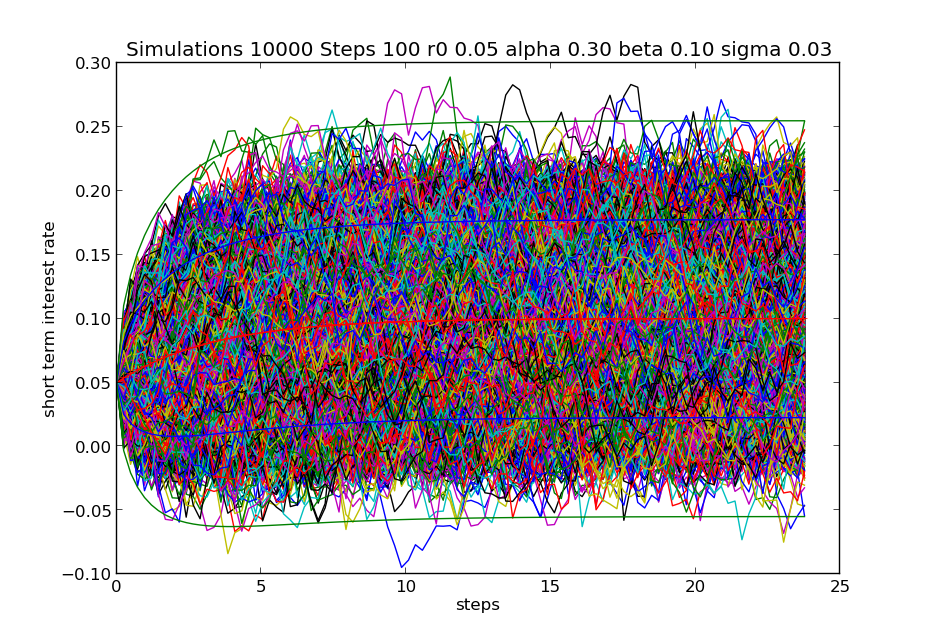
\includegraphics[bb=0 0 672 459,scale=0.5]{monte_carlo_simulation_interestrates.png}
 % monte_carlo_simulation_interestrates.png: 933x638 pixel, 100dpi, 23.70x16.21 cm, bb=0 0 672 459
\end{center}
\chapter{Examples of Interest Rate Models}
We already introduced the Vasicek model \cite{vasicek_s_model}, the dynamics
of the Vasicek model \cite{vasicek_short_rate_dynamics}and the PDE approach to the Vasicek model\cite{sub:pde_approach_to_vasicek_s_model}
 It is commonplace when studying Short rate models, to have to solve a PDE. 
Let us reintroduce in a slightly different notation, the Vasicek model. 
\begin{align*}
 dr(t) = d(t, r(t))dt + \sigma (t, r_{t}) \underbrace{Brownian Motion}{dW^*_t}, \; \forall s \geq 0 \\
r(s) = x \text{deterministic initial condition} \forall t \geq s
\end{align*}
This equation takes values in $Z = \Rbb$ or $Z = \Rbb_+$. 
\begin{note}
 You may note that we will run into a problem here, in our previous course on Stochastic Calculus, we didn't introduce 
a Stochastic Differential Equation Framework, something to handle $\Rbb_+$
\end{note}
\begin{equation*}
 r(t) = r(s) + \int_s^t (b(u), r(u))du + \int_s^t \sigma (u, r_u)dW^*_u
\end{equation*}
\begin{equation*}
\text{Assumptions} \forall s \geq 0
\begin{cases} dr_t = b(t,r_t)dt + \sigma(t, r_t) \underbrace{\text{Brownian Motion w.r.t. EMM$\Qbb$}}{dW^*_t} 
\\
r_s = x (\in Z); & t \geq s
\end{cases}
\end{equation*}
has a unique solution $\forall x \in Z$, with values in Z.
\end{document}